\documentclass[11pt]{article}
\usepackage[margin=0.85in]{geometry}
\usepackage{amsmath,amssymb,amsthm,booktabs,graphicx,microtype,hyperref,enumitem,xcolor}
\hypersetup{colorlinks=true,linkcolor=blue!55!black,citecolor=blue!55!black,urlcolor=blue!55!black}
\newtheorem{proposition}{Proposition}
\newtheorem{definition}{Definition}
\newcommand{\tr}{\operatorname{tr}}
\newcommand{\Gr}{\operatorname{Gr}}
\newcommand{\Id}{I}
\title{Elemental Peeling and What the Boundary Retains\\[4pt]\large Subspace Geometry, Optical Response, and Predictive Information}
\author{Jeromie N. Beasley\\\small Operator-first research programme}
\date{Combined research manuscript 1.0 --- 8 September 2026}
\begin{document}
\maketitle
\begin{abstract}
A peeling process can remove material, change electronic coupling, or merely shorten an effective description. These operations can produce similar scalar observations while retaining different information about the next response. We combine the hypersurface, projector, scale, and optical strands of the operator-first programme into a finite observation framework. Exact elimination places the hidden sector in a boundary self-energy; elastic contacts produce a unitary scattering matrix; its graph defines an orthogonal projector on a Grassmannian. The full graph retains the amplitude operator, while a fixed-reference principal-angle compression identifies conjugate boundary phases. An explicit two-orbital pair realizes this ambiguity: both members have conductance $G_0/2$, Fano factor $1/2$, and the same isolated optical transition gap and strength, yet their conductance slopes are opposite. At a probe displacement of one tenth of the reference energy, their transmissions are $8100/19981$ and $12100/20021$. We prove a corresponding limit on prediction from the common scalar record. Evaluated Cu/Ag/Au/Pt ionization sequences and published optical constants provide separate elemental calibrations. The combined contribution is a reproducible intervention-discrimination framework and exact benchmark, not a measured atom-by-atom cascade or a universal elemental law. The supplement separates written proofs, finite computations, pinned formal certificates, and physical assumptions.
\end{abstract}

\section{One material, several records}
An elemental peel should answer a physical question: what changed in the specimen, and what information about that change remains accessible? Electron emission, thinning a film, stretching a metallic contact, reducing an orbital coupling, and eliminating coordinates in a calculation need not have the same answer. Conductance, color, a spectral gap, and a subspace angle are observations of different aspects of that process. Agreement in one does not establish equivalence of the underlying states.

The present manuscript joins two previously separate lines. The peeling draft distinguished channel loss, coordinate elimination and signal disappearance. The light and hypersurface drafts described projector geometry, phase records and response at an interface. Their shared question is predictive: when two stages look identical through an available observation, does a richer retained record distinguish their subsequent responses? We use the actual \emph{Matter at a Scale} v5, \emph{The Soficity Trace}, \emph{Universal Projector Geometry from Electrical Measurements} v2, and \emph{Light Keeps the Ledger}, research edition 4, as source documents \cite{matter,sofic,upg,light}. Appendix A identifies the passages used and the corrections retained.

The phrase ``space of subspaces'' has a precise meaning here. A physical boundary model, together with fixed ports and a measurement convention, determines a map into a Grassmannian. We construct that map. Its existence does not mean that a physical surface creates the abstract Grassmannian, nor does it identify a material interface with a Fermi surface or an atomic shell. Each space and each derivative must be specified.

The main benchmark is deliberately small enough to solve exactly. It establishes an identifiable failure of reduced observations before any attempt to fit a material. The elemental comparisons then calibrate what actual data can enter this framework. This order keeps a mathematical demonstration distinct from a proposed physical explanation.

\section{Interventions, references and subspaces}
\begin{definition}[A recorded peeling process]
A finite peeling process consists of a parameter $\lambda$, a physical intervention, an electronic model $H_\lambda$, a preparation, contacts or optical boundaries, and observation maps. The record includes the parameter units, the orbital and port conventions, and the criterion used to select a subspace. A physical elemental peel additionally specifies the species, constituent change, geometry and environment.
\end{definition}

We distinguish three mechanisms. A positive-channel peel changes nonnegative weights of fixed transition vectors. An orbital or geometric peel changes the Hamiltonian and usually the transition vectors. A coordinate peel retains a smaller state space while incorporating eliminated coordinates through an exact effective operator. A measured decrease may also arise from changed interference or preparation without any of these removals.

\subsection{What Matter contributes: zero, span and a reference}
For a Hermitian $H$, an affine change $H'=aH+bI$, $a>0$, preserves its eigenspaces when the same spectral cluster is selected. Projector relations therefore survive this change. A laboratory energy reference is additional data. If the chemical potential is kept fixed while $H$ changes, occupation can change; this is not a change of units. In an open model with contact amplitude matrix $W$, consistent energy rescaling requires
\begin{equation}
 H'=aH+bI,\qquad E'=aE+b,\qquad W'=\sqrt a\,W.
 \label{eq:affine}
\end{equation}
The scattering response defined below is then unchanged. Substitution factors $a$ from its inverse and proves the claim. Our numerical controls test all three transformations together.

The two-sided boundary census in Matter is also retained as a specific observable, not identified with rank or electron number. For a positive contraction $C$ and $0<\epsilon<1/2$, let $N_\epsilon(C)$ count eigenvalues in $[\epsilon,1-\epsilon]$. The example
\begin{equation}
C_0=\operatorname{diag}(0.99,0.5,0.01),\quad
C_1=\operatorname{diag}(0.8,0.4,0)
\end{equation}
satisfies $0\preceq C_1\preceq C_0$, while $N_{0.1}$ increases from one to two. The underlying rank decreases. Each is a legitimate projector compression through the dilation
$\left(\begin{smallmatrix}C&\sqrt{C(I-C)}\\\sqrt{C(I-C)}&I-C\end{smallmatrix}\right)$.
Thus a threshold census can reveal a changing boundary window without counting removed constituents. Matter's ultraviolet logarithmic coefficient belongs to its specified substrate and counting convention; we do not transfer that coefficient to a metal contact.

\subsection{Positive-channel removal has a narrower theorem}
\begin{proposition}[Fixed-channel filtration]
Let $G_\lambda=\sum_j w_j(\lambda)v_jv_j^\dagger$, with fixed vectors $v_j$ and nonnegative weights that decrease along the intervention. Then $G$ decreases in positive-semidefinite order, its kernels increase by inclusion, and its rank cannot increase. Strictly positive reweighting with fixed support preserves the kernel.
\end{proposition}
\begin{proof}
For any probe $u$, $u^\dagger G_\lambda u=\sum_jw_j|v_j^\dagger u|^2$. The sum vanishes exactly when every active amplitude vanishes. Taking a difference proves the operator order, and the kernel statement follows.\end{proof}
This standard positive-form argument is the formal core of the earlier peel module. It does not apply when relaxation or interference changes the remaining amplitudes. An orbital removal can therefore increase current without contradicting this proposition.

\section{From the hypersurface to a Grassmannian}
\subsection{Exact elimination and the UPG coupling}
Split a finite Hermitian model into retained and hidden coordinates,
\begin{equation}
H=\begin{pmatrix}A&B\\B^\dagger&D\end{pmatrix},\quad
R_P=\begin{pmatrix}I&0\\0&0\end{pmatrix}.
\end{equation}
Where $EI-D$ is invertible, the retained resolvent is the inverse of
\begin{equation}
K_\Sigma(E)=EI-A-B(EI-D)^{-1}B^\dagger.
\label{eq:schur}
\end{equation}
This is the Feshbach--Schur reduction \cite{feshbach}. Solving the hidden equations and substituting into the retained equations proves it directly. Nested elimination gives the same final response whenever its pivots exist. A singular pivot is a limitation of that reduction chart; the full response may remain regular.

The UPG redistribution operator is
\begin{equation}
F(H,R_P)=(I-R_P)HR_P+R_PH(I-R_P)
=\begin{pmatrix}0&B\\B^\dagger&0\end{pmatrix}.
\end{equation}
It vanishes exactly when $[H,R_P]=0$. For $i\dot\psi=H\psi$ in units $\hbar=1$, elimination gives
\begin{equation}
\dot x(t)=-iAx(t)-iBe^{-itD}y(0)
-\int_0^t Be^{-i(t-u)D}B^\dagger x(u)\,du.
\label{eq:memory}
\end{equation}
Here the kernel at zero is $BB^\dagger$. Consequently, under Hermiticity and an orthogonal split, $F=0$ if and only if the feedback kernel vanishes identically. The forward implication is immediate; the reverse follows at $t=0$ because $BB^\dagger=0$ implies $B=0$. Hidden initial preparation is a separate retained term in Eq.~\eqref{eq:memory}. This is effective memory caused by partial observation, not by itself a non-Markovianity witness or a topological memory field.

\subsection{An explicitly contacted boundary}
Let $W$ map $m$ lead channels into the finite electronic space. Assume elastic, lossless scattering with the wide-band contact self-energy and fixed channel reference planes. For real $E$ define
\begin{equation}
R(E)=\left(EI-H+\frac{i}{2}WW^\dagger\right)^{-1},\qquad
S(E)=I-iW^\dagger R(E)W.
\label{eq:scattering}
\end{equation}
These equations supply a declared microscopic-to-boundary model; they are not an inference from a measured covariance matrix. Ports supported on the retained sector permit Eq.~\eqref{eq:schur} to be inserted without changing $S$.

\begin{proposition}[Boundary graph lift]
Where the inverse in Eq.~\eqref{eq:scattering} exists, $S$ is unitary. The matrix
\begin{equation}
\mathcal P_S=\frac12\begin{pmatrix}I&S^\dagger\\S&I\end{pmatrix}
\label{eq:graph}
\end{equation}
is a rank-$m$ orthogonal projector, and for unitary $S,T$ on the same ports,
\begin{equation}
\|\mathcal P_S-\mathcal P_T\|_F^2=\frac12\|S-T\|_F^2.
\label{eq:graphdistance}
\end{equation}
The graph determines $S$ exactly through twice its lower-left block.
\end{proposition}
\begin{proof}
The inverse identity gives $R^\dagger-R=iR^\dagger WW^\dagger R$. Expanding $S^\dagger S$ cancels the two nonidentity terms. With $Q_S=(I,S)^\mathsf T/\sqrt2$, $Q_S^\dagger Q_S=I$ and $\mathcal P_S=Q_SQ_S^\dagger$, proving the projector and rank assertions. The two off-diagonal blocks of a graph difference are $(S-T)/2$ and its adjoint; summing their squared norms proves Eq.~\eqref{eq:graphdistance}.\end{proof}

Thus $\lambda\mapsto\mathcal P_{S_\lambda}\in\Gr(m,2m)$ is the promised map from a specified boundary evolution to a space of subspaces. It is smooth wherever the underlying model is smooth and its full inverse is regular. Its rank remains $m$ even when individual transmitting channels close. An occupied electronic projector, a transmission-eigenchannel projector, and this graph projector are different objects. A common fixed change of port bases acts by a common unitary conjugation of their graph representations and preserves the distance. Uncalibrated changes of phase reference between snapshots cannot be interpreted as physical motion.

\subsection{What the angle compression forgets}
Let $\mathcal P_I$ be the graph projector of the identity reference. Then
\begin{equation}
Q_S^\dagger(I-\mathcal P_I)Q_S
=K_S:=\frac{2I-S-S^\dagger}{4}.
\label{eq:compression}
\end{equation}
The eigenvalues of $K_S$ are squared principal sines. This follows from
$Q_I^\dagger Q_S=(I+S)/2$. In particular,
\begin{equation}
 K_S=K_{S^\dagger},
\end{equation}
although their complete graph projectors can differ. On the nonfixed sector, the Cayley coordinate $Z=(I+S)(I-S)^{-1}=iX$, with $X=X^\dagger$, gives $K_S=(I+X^2)^{-1}$. Squaring has removed the sign of $X$. The fixed sector is excluded only from this Cayley chart, not from the full graph.

These identities were already present in the light draft for general unitaries. Their role here is a concrete realization by a contacted electronic model. The Sofic ancestry also matters: for permutation matrices, normalized Hamming distance equals $n^{-1}\|\mathcal P_U-\mathcal P_V\|_F^2$. That exact conversion does not transfer operator-norm stability or a winding obstruction to normalized Hamming distance. We retain the original distinction between an operator, its defect spectrum, and its scalar norm.

\section{An exact witness of lost predictive information}
Consider two noninteracting, spin-degenerate two-orbital models in units where each lead width is one:
\begin{equation}
H_s=\begin{pmatrix}0&1\\1&s\end{pmatrix},\quad s\in\{+1,-1\},\qquad
W=\begin{pmatrix}1&1\\0&0\end{pmatrix}.
\label{eq:twins}
\end{equation}
Both leads contact the first orbital. The second is side-coupled. The energy zero is the same lead reference in both preparations. Direct inversion gives
\begin{equation}
\mathcal T_s(x)=\frac{(x-s)^2}{(x^2-sx-1)^2+(x-s)^2}
=\frac{(x-s)^2}{x^4-2sx^3+2}.
\label{eq:twinT}
\end{equation}
The second equality uses $s^2=1$. The sum-of-squares denominator is strictly positive on the real line: if $x-s=0$, the other squared term is one. The transmission therefore remains regular at the side-orbital Schur pole $x=s$, where it vanishes.

\begin{proposition}[Equal reduced readings, different responses]
The pair in Eq.~\eqref{eq:twins} has the following properties:
\begin{enumerate}[nosep]
\item At $x=0$, both have $G/G_0=\mathcal T=1/2$ and zero-temperature, low-bias Fano factor $1-\mathcal T=1/2$.
\item Their isolated Hamiltonians have the same transition gap $\sqrt5$ and squared dipole strength $1/5$ for $D=\operatorname{diag}(1,0)$.
\item Their entire fixed-reference matrices $K_S$ agree, but their scattering graph projectors have squared Frobenius distance two.
\item Their energy slopes are $\mathcal T'_s(0)=-s$; at $x=1/10$,
\begin{equation}
\mathcal T_+(1/10)=\frac{8100}{19981}=0.405385\ldots,\qquad
\mathcal T_-(1/10)=\frac{12100}{20021}=0.604365\ldots.
\end{equation}
\end{enumerate}
\end{proposition}
\begin{proof}
Equation~\eqref{eq:twinT} gives the initial and displaced transmissions. Its derivative at zero is $-s$. Completing the characteristic polynomial gives eigenvalues $(s\pm\sqrt5)/2$. The two-level spectral projectors, or direct normalized eigenvectors, give $|\langle +|D|-\rangle|^2=1/(s^2+4)=1/5$.

At zero energy the full matrices are
\begin{equation}
S_+=\frac12\begin{pmatrix}1-i&-1-i\\-1-i&1-i\end{pmatrix},\qquad
S_-=S_+^\dagger,
\end{equation}
so both give $K_S=\tfrac14\left(\begin{smallmatrix}1&1\\1&1\end{smallmatrix}\right)$. Their difference has four entries of modulus one. Equation~\eqref{eq:graphdistance} gives squared graph distance two.\end{proof}

The absolute isolated spectra differ in their centers. This is not a claim of identical full spectra at fixed chemical potential. The equal optical information is the isolated transition gap and matrix element; a complete contacted optical spectrum with relaxation and lead occupations has not been shown equal. Within the stated isolated preparation, the same gap and positive transition residue give the same lossless polarizability. The contacted electrical measurement is separately specified. These distinctions prevent a narrow equality from becoming an unsupported claim of complete observational equivalence.

The occupied-projector squared distance is $2/5$, despite the equal gap and optical strength. For a normalized traceless two-level Hamiltonian, the two unit Bloch vectors have dot product $3/5$, yielding occupied overlap $4/5$ and principal angle $\arccos\sqrt{4/5}=26.565\ldots$ degrees. Thus the UPG/Grassmannian record also distinguishes the preparations, provided the orbital reference and preparation are physically calibrated.

\begin{proposition}[A limit on prediction from the common record]
Let a measurement map assign the same record to the two models, and let a deterministic predictor use only that record to predict their transmission at $x=1/10$. Its maximum absolute error over the pair is at least
\begin{equation}
\frac12\left|\frac{12100}{20021}-\frac{8100}{19981}\right|
=0.09949015\ldots.
\end{equation}
\end{proposition}
\begin{proof}
The predictor must output the same number $y$ for both inputs. The triangle inequality bounds the separation of their true outputs by $|a-y|+|b-y|$, which is at most twice the larger error.\end{proof}
This elementary lower bound specifies the instrument's advantage without a claim of superiority over all competing methods. A phase-sensitive boundary measurement distinguishes this pair. Predicting an arbitrary future still requires a validated intervention model; even the full scattering matrix at one energy does not determine an arbitrary unknown internal Hamiltonian.

\subsection{A continuous paired peel and an independent readout}
Replace the off-diagonal entries in Eq.~\eqref{eq:twins} by $g>0$. At $x=0$ both members give
\begin{equation}
\mathcal T_s(0;g)=\frac1{1+g^4},\qquad
\partial_x\mathcal T_s(0;g)=
-\frac{2s g^2(1+g^2)}{(1+g^4)^2}.
\end{equation}
Their currents remain equal throughout the matched coupling peel, while their slopes keep opposite signs. Decreasing $g$ raises current toward one conductance quantum by releasing destructive interference. Fano interference and its thermoelectric consequences are established physics \cite{fano}; the contribution here is their exact role as a combined-observation benchmark.

With $t=k_BT/\gamma$ and chemical potential zero, define
$L_j=\int u^j\mathcal T_s(tu)[4\cosh^2(u/2)]^{-1}du$ for $j=0,1$.
The linear thermopower in units $k_B/e$, using positive charge magnitude $e$, is $-L_1/L_0$. Since $\mathcal T_-(x)=\mathcal T_+(-x)$, the finite-temperature conductances agree and thermopowers have opposite signs. Numerical quadrature independently confirms this symmetry. This makes thermopower an additional practical discriminant. Recent gold-contact measurements show why a constant conductance plateau need not imply a constant energy-sensitive transport state \cite{goldcontacts}. Their phonon discussion also cautions against interpreting an experimental thermopower solely through this elastic model.

\begin{figure}[t]
\centering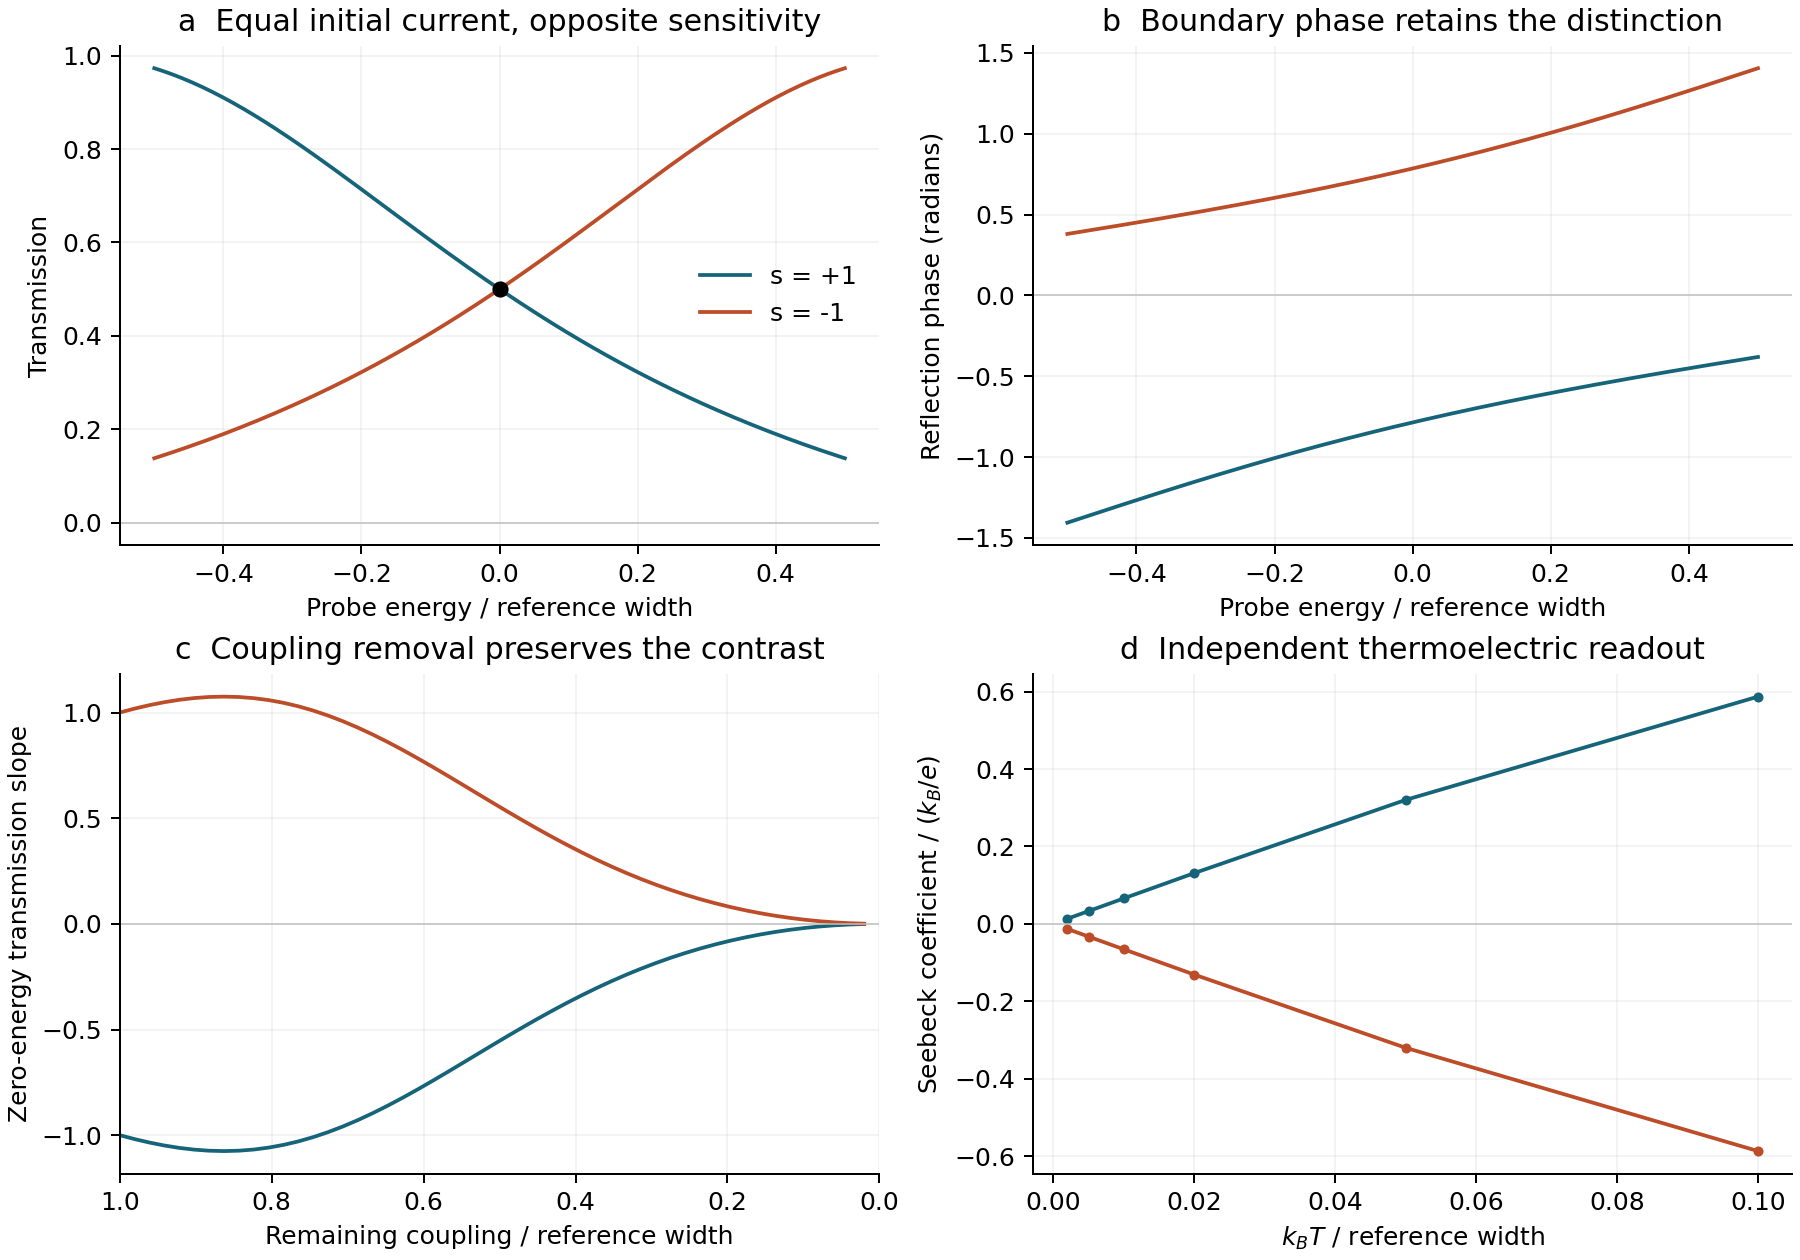
\includegraphics[width=\linewidth]{figures/predictive_pair.png}
\caption{Exact response pair. Equal zero-energy transmission hides opposite slopes. The paired coupling peel retains equal current while energy sensitivity differs. Finite-temperature integration gives equal conductance and opposite thermopower. These are specified model computations, not elemental measurements.}
\end{figure}

\section{Elemental calibrations: Cu, Ag, Au and Pt}
\subsection{Atomic spacing is one record}
The first twelve successive NIST ionization thresholds show a large later increment after eleven removals for Cu, Ag and Au, and after ten for Pt. The neutral outer configurations are respectively $3d^{10}4s^1$, $4d^{10}5s^1$, $5d^{10}6s^1$ and $5d^96s^1$. The later energy increments are 101.67, 83.46, 79.8 and 75.5 eV. Several high-charge entries are estimates; the source flags and uncertainties are preserved \cite{nist}.

This is a reproducible element-specific shell pattern, not a uniform spacing law. It does not identify isolated-ion thresholds with interband transitions or with available states near the Fermi level. The nuclear charge stays fixed: ionizing gold does not produce platinum. The comparison is useful precisely because it forces the term ``spacing'' to name its actual spectrum.

\subsection{Optical spacing, coupling and both interfaces}
Johnson--Christy's measured Au, Ag and Cu optical constants and Raki\'c's fitted Pt response give a separate visible-light comparison \cite{johnson,rakic}. Computed semi-infinite normal-incidence reflectances are:
\begin{center}
\begin{tabular}{lrrr}\toprule
Optical input & 450 nm & 550 nm & 650 nm\\\midrule
Au, measured constants & 0.408 & 0.792 & 0.957\\
Ag, measured constants & 0.980 & 0.983 & 0.990\\
Cu, measured constants & 0.538 & 0.624 & 0.935\\
Pt, fitted constants & 0.588 & 0.641 & 0.678\\\bottomrule
\end{tabular}
\end{center}
These calculated reflectances are not newly acquired measurements. The supplement also varies a smooth film's thickness from 200 to 10 nm and its transparent substrate index from one to two, keeping the material optical constants fixed. A coherent Maxwell calculation supplies reflected and transmitted power, absorption and reflected phase. CIE 1931 color matching under D65 daylight converts the reflected spectrum into a specified color observation. Independent boundary-amplitude matching and absorbed-volume Poynting integration check the calculation.

Changing thickness or substrate changes color with no alteration of the input bulk spectrum. This is the direct optical role of the hypersurface: its two sides belong to the measurement problem. At very small thickness, roughness, percolation, structural relaxation and changed electronic response require additional inputs. The model stops at 10 nm and makes no atomic-monolayer extrapolation. Optical-fit zero-frequency limits are not used as measured bulk DC conductivities.

\subsection{A shared electronic control, and its limit}
The recovered electronic-sheet model is $H_\theta=(\Delta/2)(\cos\theta\,\sigma_z+\sin\theta\,\sigma_x)$ with fixed $D=\sigma_z$. Its levels stay at $\pm\Delta/2$, while the squared dipole is $\sin^2\theta$. With separate wide-band leads on the two orbitals, the zero-energy conductance is
\begin{equation}
G/G_0=\frac{\gamma^2(\Delta/2)^2\sin^2\theta}
{[(\Delta/2)^2+\gamma^2/4]^2}.
\end{equation}
This explicitly connects orbital orientation to two readouts at fixed spacing. The scalar relation depends on the specified contact and dipole directions. The new response pair goes further by showing that even matched dipole strength and current can leave predictive information hidden.

No model here is an ab initio Hamiltonian for all four metals. Recent goldene studies already investigate strain, defect-sensitive transport, optical response and thermoelectric properties \cite{goldene,multigoldene}. A material-specific advance must therefore predict or distinguish a calibrated intervention, rather than claim novelty for combining these subjects.

\section{Physical geometry requires a physical convention}
Projector geometry and its connection to response are established subjects \cite{projector,oh,embedding}. A particularly close July 2026 preprint shows that orbital positions must be included consistently in the physical current and in the derivative used for band geometry \cite{embedding}. Our finite model fixes a physical orbital basis, a dipole and contact vectors; rotating the Hamiltonian alone is a physical model change relative to those probes. A mere change of representation transforms all of them together.

We test this distinction twice. Simultaneous transformations $H\mapsto UHU^\dagger$ and $W\mapsto UW$ leave the scattering matrix unchanged. For a parameter-dependent basis $B(k)=e^{ikX}$ and $P'=BPB^\dagger$, ordinary differentiation gives
\begin{equation}
\partial_kP'=B(\partial_kP)B^\dagger+i[X,P'].
\end{equation}
The covariant derivative $\partial_kP'-i[X,P']$ restores the original metric. A 65-point two-band control shows both the restored equality and the spurious difference obtained by omitting the connection. This checks representation covariance. It does not replace the separate derivation of the physical position operator and current in a real crystal.

The same discipline applies to a physical hypersurface. A fitted interface alone does not determine the interior Hamiltonian. Distinct interiors can share a boundary response over an insufficient probe set. The graph representation is lossless with respect to its supplied amplitude operator; it does not solve that inverse problem automatically.

\section{Reduction geometry: what the additional sources establish}
The newly supplied square-case, FOFT and singular-angle papers provide complementary controls \cite{ladder,foft,angle}. They concern different objects, but each specifies information that survives a reduction and information that must be supplied for reconstruction. This is the useful common structure; an angle in one construction is not automatically the same physical observable as an angle in another.

\subsection{Gram shape, orientation and reconstruction}
For a real square Jacobi matrix $X\ne0$ define its size $r=\|X\|_F$, normalized configuration $Y=X/r$, and Gram matrix $G=Y^\top Y$. Then $G\succeq0$, $\tr G=1$, and the generic shape dimension is $d(d+1)/2-1$. Reflection $Y\mapsto RY$, $R\in O(d)$ with $\det R=-1$, leaves $G$ fixed and reverses the signed volume. The identity
\begin{equation}
\det G=(\det Y)^2
\end{equation}
makes the lost orientation explicit. In two dimensions the rotation quotient is the familiar double of the Gram disc, giving the shape sphere. The two orientations meet on the zero-determinant locus.

The bundle statement requires two refinements to the supplied diagram. On full-rank configurations with \emph{fixed size}, the Gram map is a principal $O(d)$ bundle over the positive-definite trace-one interior. If size has not been fixed, each normalized-Gram fiber also contains positive dilations. An $SO(d)$ bundle instead uses the oriented cover as base, or one fixed orientation component. The closed positive-semidefinite base has rank strata and is not a single principal-bundle chart. For the $SO(d)$ action, a rank-$r$ configuration has stabilizer $SO(d-r)$; the orientation cover branches already at rank $d-1$, where that stabilizer is still trivial. Branching and continuous rotational isotropy are therefore distinct events.

A Gram trajectory and an initial frame determine a horizontal lift only after a connection has been specified. For arbitrary physical motion, angular momentum or vertical rotation is additional information; a mechanical horizontal lift corresponds to its stated constraint. Thus a closed shape path can carry reconstruction holonomy, but shape alone does not determine every possible physical rotation. The electronic counterpart is similarly conditional: fixed reference channels are needed before boundary phase records can be compared. This is a structural analogy, not an identification of mechanical and electronic connections.

\subsection{A singular angle is an exact restricted diagnostic}
Let $M=uv^\top$ with unit real $u,v$, so that $\|M\|_F=1$. Direct multiplication gives
\begin{equation}
MM^\top=uu^\top,\qquad M^\top M=vv^\top,\qquad
\tfrac12\|[M,M^\top]\|_F^2=1-|u^\top v|^2=\sin^2\theta.
\label{eq:singular}
\end{equation}
Here $\theta$ is the principal angle between the left and right singular lines. This is the angle insert's precise identity. Positive rescaling is invisible only after normalization; for an unnormalized rank-one matrix the stress acquires a factor $\|M\|_F^4$. Tensor products multiply direction cosines, hence $1-\Phi_{A\otimes B}=(1-\Phi_A)(1-\Phi_B)$ for normalized rank-one factors. Our controls verify both identities and reject higher-rank input to this one-angle diagnostic.

The continued-fraction interpretation $\tan\theta=|K|$ additionally requires the left singular line to approach the coordinate axis used to define $K$. The insert explicitly excludes its Ap\'ery calibration from that stronger interpretation. Likewise, a normalized transport product $M$ is not an orthogonal occupied-state projector: the latter has zero self-commutator identically. Equation~\eqref{eq:singular} shares principal-angle algebra with the graph compression while preserving its own domain.

\subsection{FOFT relaxation preserves a spectrum, not generic isotropy}
For a finite matrix $K$ set $C=[K,K^\dagger]$ and $\Phi=\|C\|_F^2/2$. FOFT's stated flow is
\begin{equation}
\dot K=-2[C,K],\qquad
\frac{d\Phi}{dt}=-4\|[C,K]\|_F^2,\qquad
\frac{d}{dt}\|K\|_F^2=-8\Phi.
\label{eq:foft}
\end{equation}
The first equation is a Lax flow, so eigenvalues remain constant. The last identity follows from cyclicity of trace: $2\operatorname{Re}\tr(K^\dagger\dot K)=-4\tr(C^2)$. Thus the Henrici budget $\|K\|_F^2-\sum_j|\lambda_j|^2$ decreases even when the spectrum is fixed. Our independent integration preserves the eigenvalues to $2.7\times10^{-12}$ while reducing the stress.

The diagonal matrix $\operatorname{diag}(1,2)$ is already a nonscalar fixed point. Normality therefore does not establish an isotropic vacuum or a common eigenvalue. The v2.2 equilibrium corollary correctly requires a fully degenerate conserved spectrum for a scalar endpoint; its abstract's unconditional isotropy statement is not used. The Frobenius dissipation in Eq.~\eqref{eq:foft} also becomes physical heat only after an energy model is supplied.

The v2.2 zero/span script uses $R R^+$ for a selected eigenvector frame $R$. This is its orthogonal range projector, not generally the oblique Riesz projector named in the comment. For example,
\begin{equation}
K=\begin{pmatrix}1&2\\0&3\end{pmatrix},\quad
P_{\mathrm{range}}=\begin{pmatrix}1&0\\0&0\end{pmatrix},\quad
P_{\mathrm{Riesz}}=\frac{3I-K}{2}=\begin{pmatrix}1&-1\\0&0\end{pmatrix}.
\end{equation}
Both select the same one-dimensional range, but only the Riesz projector commutes with $K$. Scale invariance of the selected range survives this correction. Arguments about commuting spectral projectors must use the correct object.

\subsection{The ladder carries a positive inner product}
For positive vectors $g,t$, with $\sum_i g_i=1$, put
\begin{equation}
M=\operatorname{diag}(t)-gt^\top,\quad
S=\operatorname{diag}\sqrt{g_i/t_i},\quad u_i=\sqrt{g_it_i}.
\end{equation}
Then $M=S[\operatorname{diag}(t)-uu^\top]S^{-1}$, since $Su=g$ and $u^\top S^{-1}=t^\top$. Consequently $M$ is self-adjoint for the positive weight $S^{-2}$ and has real, diagonalizable spectrum. Restriction to the invariant trace-zero tangent gives the square-case paper's eigenvalue block, with its stated factor of two. For distinct $t_i$, the positive secular weights give strict interlacing; coincident poles require the corresponding multiplicity statement.

This connects directly to the earlier skew controls: Euclidean non-normality can coexist with self-adjointness in a specified positive inner product. If a $g_i$ vanishes, this symmetrizer degenerates. That failure allows a different boundary analysis; it does not prove that every boundary point is defective. In the combined paper, singularity of a Gram chart, failure of an elimination pivot, loss of a spectral gap, and physical channel removal remain separately recorded events.

\section{Verification and a falsifiable experimental programme}
The new suite contains 550 registered-eye evaluations and 1,700 assertions, with two deliberate domain refusals. It checks 402 displaced-energy responses, a 102-frame paired coupling sweep, general unitary graph identities, representation covariance, a UPG feedback case and the exact rational witness. The previously completed elemental suite contains 1,253 evaluations, including four intended refusals, and 846 assertions. Its exact source commit is retained. The recovered hypersurface verifier passed 328 checks in that earlier run; the original color model passed as well. These are evaluation and assertion counts, not counts of independent physical experiments.

Six new immutable methods bring Compound Eye to 204 versions, preserving all previous 198. A further 340 source-control evaluations and 745 assertions check the Gram, angle, FOFT and ladder additions, with three intended domain refusals. The supplied original FOFT gradient script also completes; the large lattice scans are not represented as freshly rerun. The scientific conclusions follow from the displayed equations and inputs; the instrument coordinates the observations and retains their provenance. The new formal module covers redistribution algebra, the response rational functions, their exact equalities and counterexample, positivity and remainder identities. The general scattering/graph derivation and physical interpretation remain written mathematics. All 16 new finite declarations passed Lean compilation, the axiom audit and an independent \texttt{leanchecker} recheck at commit \texttt{3eb373797a26}; the intentionally false displaced equality was rejected. The formal predictor theorem takes initial conductance as its input; the stronger joint-record proposition has the written proof above. The proof-status file records full revisions, logs and remaining obligations.

A useful first physical programme has two stages. For a metallic contact, record displacement and geometry, low-bias conductance and shot noise, energy-dependent current, temperature and thermopower; add a calibrated phase-sensitive observation where possible. For a thinning film, record thickness and structure, DC sheet resistance, reflection/transmission or ellipsometry, and the dielectric environment. The physical model must connect these experiments before their channels are identified with one another. Initial-condition and heating controls are essential before hysteresis is interpreted as memory.

The benchmark suggests a clear success criterion: a reduced record fails to distinguish two preparations or intervention stages, while the richer record predicts a reproducible later difference within calibrated uncertainties. The null alternatives include heating, contact rearrangement, untracked chemical changes, reference drift and an inadequate model. A prediction should be made before the displaced-energy or later-stage measurement is revealed. No claimed advantage should depend on choosing the successful probe after inspecting that measurement.

\section{Conclusion}
A boundary model can induce a concrete trajectory through a space of subspaces. The complete graph projector retains its unitary amplitude operator; a squared-angle compression can erase a distinction relevant to subsequent transport. Our exact two-orbital pair makes this information loss operational and quantifies a prediction limit for the shared reduced record. Matter supplies the reference discipline, UPG supplies the coupling split, the hypersurface supplies exact reduction, and the Sofic/light work supplies the distinction between a full operator and its compressed defect.

The elemental evidence provides calibrations, not the missing physical identification. The paper's foundational claim is therefore a statement about observation and reduction: deciding what a peel removes requires an intervention model and enough retained information to distinguish later responses. Establishing an elemental removal mechanism remains a material-specific test of that framework.

\appendix
\section{Source map and corrections carried into this manuscript}
\begin{description}[style=nextline,leftmargin=0pt]
\item[Matter at a Scale, v5.] Uses the offset/span distinction and compressed-projector census. Its long-range Ising and ultraviolet coefficient calculations are source-reported here, not freshly extended. Positive energy rescaling is distinguished from moving a spectrum relative to a fixed reservoir.
\item[The Soficity Trace, 23 August 2026.] Retains winding with a branch guard, norm distinctions and the corrected $\delta+g^2\le4$ bound. The supplied source gives this bound; a retrieved summary's extra factor $1/2$ is not used. The work does not establish non-soficity. The separate Sofic--Torsion Atlas note is included as ancestry, without importing an unconstructed knot APS operator.
\item[Light Keeps the Ledger, research edition 4.] Uses its graph lift, fixed-normalization displacement Gram, Cayley sign loss, positive optical weighting and probe-completeness distinctions. The historical longer HTML is retained separately. The fixed normalization $K_U=(2I-U-U^\dagger)/4$ distinguishes a three-cycle from involutions; normalization by each specimen's maximum need not.
\item[UPG v2.] Uses the redistribution operator and projector conventions. Its printed positive gluing correction is not carried forward: for a positive Hermitian block matrix, the Schur log-determinant correction has the minus sign, $\log\det(I-C^\dagger A^{-1}C)$ after appropriate normalization. Positivity of the full block matrix is required. Its displayed path cost is not a minimum over all continuous paths.
\item[Hypersurface dossier and HYPERSURFACE-TESTS-01.] Uses electronic-sheet loading and the interior/interface/exterior reduction. Original archives and the mathematical verification record are preserved. A spatial Maxwell interface is distinguished from the electronic or scattering graph projectors.
\item[FOFT v2/v2.2, square-case ladder v4, and angle insert.] Uses isospectral non-normality relaxation, fixed-size Gram reduction, its separate orientation record, positive-metric symmetrization, and the restricted rank-one angle identity. Original PDFs, archives and diagram are preserved. Normality versus isotropy, range versus Riesz projectors, scale fixing and orientation-cover base conditions are corrected explicitly in the main text.
\item[Peeling cascade and QHE additions.] Retains positive-channel assumptions, exact elimination, hidden initial forcing, and calibrated energy bookkeeping. Multiple relaxation times alone do not demonstrate quantum memory. A peel is not called a heat engine without a work/heat ledger and a closed cycle.
\end{description}

Zenodo searches and direct attempts to read the supplied record identifiers failed or timed out during preparation. We therefore cite the actual bundled manuscript editions and do not claim that their latest public publication metadata was independently verified. GitHub branches and open pull requests were freshly inspected; original formal sources stay pinned. The supplement's source inventory provides full file hashes.

\section{Exact scalar remainder and formal scope}
For $D_s(x)=(x^2-sx-1)^2+(x-s)^2$, the identities
\begin{align}
2D_+(x)[\mathcal T_+(x)-\tfrac12+x]&=x^2(2+2x-5x^2+2x^3),\\
2D_-(x)[\mathcal T_-(x)-\tfrac12-x]&=x^2(2-2x-5x^2-2x^3)
\end{align}
hold exactly. Together with $D_s(0)=2$ and positivity, they prove the opposite slopes and an explicit quadratic remainder by ordinary continuity. The Lean source certifies these algebraic identities; it does not label a written analytic limit as a separately formalized derivative theorem. A deliberately false equality of the two displaced transmissions is included as a negative control.

\section{Reproduction}
The standalone supplement contains this manuscript source, the six new methods, the current immutable registry and implementations, input manuscripts, the elemental data and earlier elemental controls, new execution records, formal sources, source hashes and a full proof-status record. Run the supplied top-level reproduction script; it supplies the directory structure expected by the instrument. No code editing is required. The PDF and HTML are complete reading copies. Mathematical checks, data replay and formal verification have separate commands and scopes.

\begin{thebibliography}{99}
\bibitem{matter} J. N. Beasley, \emph{Matter at a Scale: Zero, Span, and the Logarithm Between Them}, v5, August 2026. User-supplied manuscript and source archive.
\bibitem{sofic} J. N. Beasley, \emph{The Soficity Trace}, 23 August 2026; \emph{Sofic--Torsion--Atlas Working Note}. Bundled source editions.
\bibitem{upg} J. N. Beasley, \emph{Universal Projector Geometry from Electrical Measurements}, v2, 2026. Bundled source; corrections in Appendix A.
\bibitem{light} J. N. Beasley, \emph{Light Keeps the Ledger: Matter, Direction, and the Wall Between Them}, research edition 4, 7 September 2026. Bundled source edition.
\bibitem{ladder} J. N. Beasley, \emph{The Square Case: Gram Reduction and Spectral Transport for $N=d+1$ Bodies}, v4, August 2026; associated Gram reconstruction infographic. Supplied editions.
\bibitem{foft} J. N. Beasley, \emph{Foundational Operator Field Theory on Stratified Manifolds}, v2 and v2.2 source bundle, August 2026. Supplied editions; corrections and scope in the main text.
\bibitem{angle} J. N. Beasley, \emph{The spectral stress is an angle}, insert for \emph{The Companion-Matrix Projector Diagnostic}, 12 August 2026. Supplied edition.
\bibitem{feshbach} H. Feshbach, Unified theory of nuclear reactions, Ann. Phys. 5, 357--390 (1958). \href{https://doi.org/10.1016/0003-4916(58)90007-1}{doi:10.1016/0003-4916(58)90007-1}.
\bibitem{fano} U. Fano, Effects of configuration interaction on intensities and phase shifts, Phys. Rev. 124, 1866 (1961). \href{https://doi.org/10.1103/PhysRev.124.1866}{doi:10.1103/PhysRev.124.1866}.
\bibitem{goldcontacts} M\"oller et al., Nonmonotonic temperature dependence of the thermopower of atomic-size gold contacts, 2026 preprint. \href{https://arxiv.org/abs/2606.12734}{arXiv:2606.12734}.
\bibitem{nist} NIST Atomic Spectra Database, ionization-energy tables for Cu, Ag, Au and Pt, retrieved 8 September 2026. \url{https://physics.nist.gov/asd}. Exact query URLs and flags in the elemental data archive.
\bibitem{johnson} P. B. Johnson and R. W. Christy, Optical constants of the noble metals, Phys. Rev. B 6, 4370 (1972). \href{https://doi.org/10.1103/PhysRevB.6.4370}{doi:10.1103/PhysRevB.6.4370}.
\bibitem{rakic} A. D. Raki\'c et al., Optical properties of metallic films for vertical-cavity optoelectronic devices, Appl. Opt. 37, 5271--5283 (1998). \href{https://doi.org/10.1364/AO.37.005271}{doi:10.1364/AO.37.005271}.
\bibitem{goldene} G. R. Berdiyorov and B. Aissa, Robust conductivity of goldene against structural defects and mechanical deformations: a first-principles study, npj 2D Mater. Appl. 10, 20 (2026). \href{https://doi.org/10.1038/s41699-025-00657-y}{doi:10.1038/s41699-025-00657-y}.
\bibitem{multigoldene} K. Kumar, A. Dhasmana and A. K. Mishra, A multifunctional 2D goldene monolayer with strain-sensitive optoelectronic and thermoelectric properties, Sci. Rep. 16, 16683 (2026). \href{https://doi.org/10.1038/s41598-026-47366-0}{doi:10.1038/s41598-026-47366-0}.
\bibitem{projector} J. Mitscherling et al., Gauge-invariant projector calculus for quantum state geometry and applications to observables in crystals, Phys. Rev. B 112, 085104 (2025). \href{https://doi.org/10.1103/qscv-qxqt}{doi:10.1103/qscv-qxqt}.
\bibitem{oh} C.-G. Oh et al., Mass-invariant universal optical conductivity from quantum geometry, Sci. Adv. 12, eady2033 (2026). \href{https://doi.org/10.1126/sciadv.ady2033}{doi:10.1126/sciadv.ady2033}.
\bibitem{embedding} C.-G. Oh and S. Murakami, Orbital embedding and the physical definition of quantum geometry, 24 July 2026 preprint. \href{https://arxiv.org/abs/2607.21882}{arXiv:2607.21882}.
\end{thebibliography}
\end{document}
